\chapter{Números complejos}\label{numcomp}

Los números complejos son una extensión de los números reales que surgieron de la necesidad de calcular todas las raíces de un polinomio y darle sentido al Teorema Fundamental del Álgebra, el cual establece que todo polinomio de grado $n$ tiene exactamente $n$ raíces contando multiplicidades. Su aplicación es esencial en matemáticas, física e ingeniería. Este capítulo presenta su definición, propiedades básicas y su relación con el Teorema Fundamental del Álgebra.

\section{Propiedades básicas}

\begin{definition}[Número complejo]
Un número complejo es un número de la forma $$z=x+iy$$ donde $x$ y $y$ son números reales e $i$ es la unidad imaginaria definida como $i^2=-1$. El valor $x$ se denomina \textbf{parte real} y el valor $y$ \textbf{parte imaginaria}. El conjunto de todos los números complejos se denota por $\mathbb{C}$.
\end{definition}

\begin{rem} 
En ingeniería, la unidad imaginaria suele representarse como $j$ en lugar de $i$. Esta diferencia es puramente notacional. En este texto se utiliza la convención matemática $i$ para la unidad imaginaria.
\end{rem}

En este capítulo se estudiarán las propiedades básicas de los números complejos y su representación geométrica en el plano complejo. Se inicia con la definición de las operaciones básicas:

\begin{definition}[Operaciones básicas]
Sean $z_1=x_1+iy_1$ y $z_2=x_2+iy_2$ números complejos, se definen:
\begin{itemize}
\item \textbf{Suma:} $z_1+z_2=\left( x_1+x_2 \right) + i\left( y_1+y_2 \right)$.
\item \textbf{Multiplicación:} $z_1z_2=\left(x_1x_2-y_1y_2\right)+i\left(x_1y_2+x_2y_1\right)$.
\item \textbf{Conjugado:} $\overline{z_1}= x_1-iy_1$. En algunos textos avanzados, el conjugado se denota por $z^{*}$. Para evitar confusiones, aquí se usará la notación con línea superpuesta.
\end{itemize} 
\end{definition}

Estas operaciones dotan a los números complejos de la estructura de \textbf{campo}, fundamental para espacios vectoriales (ver Definición \ref{defespvectorial}). La demostración de las siguientes propiedades se propone como ejercicio.

\begin{theorem}[Propiedades de campo de los números complejos]
Sean $z_1,z_2$ y $z_3 \in \mathbb{C}$, entonces:
\begin{enumerate}[$1.$]
\item \textbf{Cerradura bajo la suma y la multiplicación:} $z_1+z_2$ y $z_1z_2$ $\in \mathbb{C}$.
\item \textbf{Asociatividad:} $\left(z_1+z_2 \right)+z_3=z_1+\left( z_2+z_3 \right)$ y $\left( z_1z_2 \right)z_3=z_1\left( z_2z_3 \right)$. 
\item \textbf{Elementos neutros:} Existen $\mathbf{0}=0+0i$ y $1=1+0i \in \mathbb{C}$ tales que $z_1+\mathbf{0}=z_1$ y $1 \cdot z_1=z_1$.
\item \textbf{Inversos:} Existe $-z_1=-x_1-iy_1 \in \mathbb{C}$ tal que $z_1+(-z_1)=\mathbf{0}$. Si $z_1\neq \mathbf{0}$, existe $z_1^{-1}=\dfrac{x_1}{x_1^2+y_1^2}-i\dfrac{y_1}{x_1^2+y_1^2}\in \mathbb{C}$ tal que $z_1z_1^{-1}=1$.
\item \textbf{Distributividad:} $z_1(z_2+z_3)=z_1z_2+z_1z_3$.
\end{enumerate}
\end{theorem}

\begin{prob}  (\cite{andreescu2014complex}, p. 19, Problema 1) Considere los complejos $z_1=1+2i$, $z_2=-2+3i$ y $z_3=1-i$. Calcule:
\begin{multicols}{2}
\begin{enumerate}[$(a)$]
\item $z_1+z_2+z_3$.
\item $z_1z_2z_3$.
\item $\dfrac{z_1^2 + z_2^2}{z_2^2+z_3^2}$.
\item $z_1^2 + z_2^2 +z_3^2$.
\end{enumerate}
\end{multicols}
\begin{myproof}	
$(a)$ Sumando las partes reales e imaginarias:
\begin{equation}
z_1+z_2+z_3 = (1+2i)+(-2+3i)+(1-i)=(1-2+1)+(2+3-1)i= \boxed{0+4i}.
\end{equation}

$(b)$ Calculando paso a paso y utilizando $i^2=-1$:
\begin{align*}
z_1z_2z_3 &= (1+2i)(-2+3i)(1-i)\\
&= (-2+3i+4i+6i^2)(1-i)\\
&= (-2+3i+4i-6)(1-i)\\
&= (-8+7i)(1-i)\\
&= -8+8i+7i^2-7i\\
&= -8+8i-7-7i\\
&= \boxed{-15+i}
\end{align*}

$(c)$ Calculando cada término:
\begin{align*}
z_1^2 &= (1+2i)^2 = 1+4i+4i^2 = 1+4i-4 = -3+4i\\
z_2^2 &= (-2+3i)^2 = 4-12i+9i^2 = 4-12i-9 = -5-12i\\
z_3^2 &= (1-i)^2 = 1-2i+i^2 = 1-2i-1 = -2i
\end{align*}

Por lo tanto:
\begin{align*}
\dfrac{z_1^2 + z_2^2}{z_2^2+z_3^2} &= \dfrac{(-3+4i) + (-5-12i)}{(-5-12i)+(-2i)}\\
&= \dfrac{-8-8i}{-5-14i}\\
\end{align*}

Multiplicando numerador y denominador por el conjugado del denominador:
\begin{align*}
\dfrac{-8-8i}{-5-14i} &= \dfrac{(-8-8i)(-5+14i)}{(-5-14i)(-5+14i)}\\
&= \dfrac{40+112i+40i-112i^2}{25+70i-70i-196i^2}\\
&= \dfrac{40+152i+112}{25+196}\\
&= \dfrac{152+152i}{221}\\
&= \boxed{\frac{152}{221}+\frac{152}{221}i}
\end{align*}

$(d)$ Utilizando los cálculos previos:
\begin{align*}
z_1^2 + z_2^2 +z_3^2 &= (-3+4i) + (-5-12i) + (-2i)\\
&= -8-10i
\end{align*}
\end{myproof}
\end{prob}

\begin{prob} Demuestre que $z$ es real si y solo si es igual a su conjugado.

\begin{myproof}	
Sea $z=a+bi$ un número complejo, donde $a$ y $b$ son números reales. El conjugado de $z$ es $\overline{z}=a-bi$. 

$(\Rightarrow)$ Si $z$ es real, entonces $z=a$ con $b=0$. Por tanto, $\overline{z}=a-0i=a=z$.

$(\Leftarrow)$ Si $z=\overline{z}$, entonces $a+bi=a-bi$. Esto implica que $2bi=0$, lo que solo es posible si $b=0$. Por lo tanto, $z=a$ es un número real.

En conclusión, $z$ es real si y solo si $z=\overline{z}$.
\end{myproof}
\end{prob}


\begin{prob} (\cite{andreescu2014complex}, p. 19, Problema 9) Encuentre los números reales $x,$ $y$ tales que $\dfrac{x-3}{3+i}+\dfrac{y-3}{3-i}=i.$
\begin{myproof}	
Multiplicando ambos lados por el denominador común $(3+i)(3-i)=9+1=10$:
\begin{align*}
\dfrac{x-3}{3+i}+\dfrac{y-3}{3-i}&=i\\
(x-3)(3-i)+(y-3)(3+i)&=10i\\
3x-xi-9+3i+3y+yi-9-3i&=10i\\
(3x+3y-18)+i(-x+y)&=10i
\end{align*}

Igualando partes reales e imaginarias:
\begin{align*}
3x+3y-18&=0\\
-x+y&=10
\end{align*}

De la segunda ecuación: $y=10+x$. Sustituyendo en la primera:
\begin{align*}
3x+3(10+x)-18&=0\\
3x+30+3x-18&=0\\
6x+12&=0\\
6x&=-12\\
x&=-2
\end{align*}

Por lo tanto, $\boxed{x=-2}$ y $\boxed{y=10+(-2)=8}$.
\end{myproof}
\end{prob}

La forma presentada anteriormente se denomina \textbf{forma binomial} o \textbf{cartesiana} de un número complejo. También es posible representar un número complejo como una pareja ordenada $(x,y)$ de números reales, donde la parte real se grafica en el eje $X$ y la parte imaginaria en el eje $Y$. Esta es conocida como la \textbf{representación geométrica} del complejo $z$.

\begin{prob} Calcule la representación geométrica del complejo $z=-5-4i.$ \label{formageometrica54i}
\begin{myproof} 
La parte real del complejo $z$ es $-5$ y la parte imaginaria es $-4$. Por tanto, $z$ corresponde al punto $(-5,-4)$ en el plano complejo. Su representación geométrica es:

\begin{figure}[H]
\centering
\begin{tikzpicture}[line cap=round,line join=round,>=triangle 45,x=0.5cm,y=0.5cm]
\begin{axis}[
x=0.5cm,y=0.5cm,
axis lines=middle,
ymajorgrids=true,
xmajorgrids=true,
xmin=-6.00,
xmax=2.5,
ymin=-4.74,
ymax=1.02,
xtick={-6.0,-5.0,...,1.0},
ytick={-4.0,-3.0,...,1.0},]
\clip(-6.,-4.74) rectangle (1.56,1.02);
 
\draw [fill=red!85!black] (-5.,-4.) circle (2.5pt);
\draw[color=red!85!black] (-4.86,-3.63) node {$z=-5-4i$};
 \draw[color=black] (0.8,-0.5) node {Eje Real};
 \draw[color=black] (-2,0.5) node {Eje Imaginario};
\end{axis}
\end{tikzpicture}
\caption{Representación geométrica del complejo $-5-4i.$}
\end{figure}
\end{myproof}
\end{prob} 

Haciendo uso de las coordenadas polares, podemos obtener otra representación del número complejo $z$:

\begin{definition}[Módulo y argumento]\label{modnumcom}
Sea $z=x+iy$ un número complejo, y $P$ el punto en el plano cartesiano que lo representa. El \textbf{módulo} de $z$, denotado por $\abs{z}$, es la distancia desde el origen $O$ hasta el punto $P$, dado por $\abs{z}=\sqrt{x^2+y^2}$. El \textbf{argumento} de $z$, denotado por $\text{arg}(z)$, es el ángulo medido desde la parte positiva del eje real hasta el segmento $\overline{OP}$. Aunque el argumento puede tomar cualquier valor que difiera en múltiplos de $2\pi$, se suele considerar el \textbf{argumento principal} en el intervalo $[0,2\pi)$.
\end{definition}

Antes de presentar la forma polar, introducimos una de las fórmulas más importantes en matemáticas, cuya demostración se hará en el Teorema \ref{demformeuler}.

\begin{theorem}[Fórmula de Euler]\label{formeuler} Para cualquier número real $\theta$:
$$\mathrm{e}^{i\theta}=\cos \theta + i \sen \theta.$$
\end{theorem}

\begin{definition}[Forma polar] 
Sea $z=x+iy$ un número complejo con módulo $\abs{z}$ y argumento $\theta=\text{arg}(z)$. La forma polar de $z$ se expresa como:
$$z=\abs{z}\mathrm{e}^{i\theta}.$$
\end{definition}

Una ventaja significativa de la forma polar es la simplificación de las operaciones de multiplicación y división:

\begin{theorem}[Multiplicación y división en forma polar]
Sean $z_1=\abs{z_1}\mathrm{e}^{i\theta_1}$ y $z_2=\abs{z_2}\mathrm{e}^{i\theta_2}$ números complejos. Entonces:
\begin{enumerate}[$1.$]
\item $z_1z_2=\abs{z_1}\abs{z_2}\mathrm{e}^{i(\theta_1 + \theta_2)}.$
\item $\dfrac{z_1}{z_2}=\dfrac{\abs{z_1}}{\abs{z_2}}\mathrm{e}^{i(\theta_1 - \theta_2)}.$
\end{enumerate}
\end{theorem}

\begin{rem} 
De este teorema se deduce que multiplicar complejos en forma polar equivale a multiplicar sus módulos y sumar sus argumentos, mientras que dividir complejos equivale a dividir sus módulos y restar sus argumentos. Para estas operaciones es importante considerar el cuadrante y posiblemente ajustar para obtener el argumento principal.
\end{rem}

\begin{prob} Encuentre la forma polar del número complejo $z=-5-4i.$ ¿Cuál es el efecto geométrico en el plano complejo de multiplicar y dividir por este número? Justifique su respuesta. \label{formapolar54i}

\begin{myproof}
Para encontrar la forma polar de $z=-5-4i$, calculamos:

El módulo: $|z|=\sqrt{(-5)^2+(-4)^2}=\sqrt{25+16}=\sqrt{41}$.

Para el argumento, calculamos $\tan\theta = \frac{-4}{-5}=\frac{4}{5}$, lo que da $\theta = \arctan\left(\frac{4}{5}\right) \approx 0.6747$ radianes. Como $z$ se encuentra en el tercer cuadrante (tanto $x$ como $y$ son negativos), debemos sumar $\pi$ al valor obtenido:
$$\text{arg}(z) = \pi+\arctan\left(\frac{4}{5}\right) \approx 3.8163 \text{ radianes}.$$

Por tanto, la forma polar de $z$ es $\boxed{z=\sqrt{41}\,\mathrm{e}^{i\cdot 3.8163}}$.

Respecto al efecto geométrico:
- Multiplicar un número complejo por $z$ tiene dos efectos: (1) una dilatación por un factor de $\sqrt{41} \approx 6.40$ y (2) una rotación en sentido antihorario de aproximadamente $3.8163$ radianes (218.8°).
- Dividir por $z$ produce: (1) una contracción por un factor de $\frac{1}{\sqrt{41}} \approx 0.156$ y (2) una rotación en sentido horario de $3.8163$ radianes.
\end{myproof}
\end{prob}

Es posible verificar los resultados de los problemas \ref{formageometrica54i} y \ref{formapolar54i} mediante el siguiente programa en \texttt{Python 3.x}:

\begin{prob} Use el lenguaje de programación \texttt{Python 3.x} para calcular la forma geométrica y polar del número complejo $-5-4i$.
\begin{myproof}
\begin{lstlisting}[label={lst:complejo},basicstyle=\footnotesize]
import cmath
import matplotlib.pyplot as plt

def calcular_modulo_argumento(numero_complejo):
    modulo = abs(numero_complejo)
    argumento = cmath.phase(numero_complejo)
    
    # Normalizar el argumento al intervalo [0, 2π)
    if argumento < 0:
        argumento += 2 * cmath.pi
    elif argumento > 2 * cmath.pi:
        argumento %= 2 * cmath.pi
    
    return modulo, argumento

# Entrada de valores
real_part = float(input("Parte real: "))
imag_part = float(input("Parte imaginaria, sin la i: "))
numero_complejo = complex(real_part, imag_part)

# Cálculo de módulo y argumento
modulo, argumento = calcular_modulo_argumento(numero_complejo)
print(f'Módulo: {modulo}')
print(f'Argumento: {argumento} radianes')

# Visualización gráfica
plt.figure(figsize=(8, 8))
plt.scatter(real_part, imag_part, color='red', marker='x', label='Número complejo')
plt.xlabel('Parte Real')
plt.ylabel('Parte Imaginaria')
plt.title('Representación en el Plano Complejo')
plt.axhline(0, color='black', linewidth=0.5)
plt.axvline(0, color='black', linewidth=0.5)
plt.grid(color='gray', linestyle='--', linewidth=0.5)
plt.legend()
plt.show()
\end{lstlisting}

Este programa genera la siguiente salida:

Parte real: -5

Parte imaginaria, sin la i: -4

Módulo: $6.4031242374328485$

Argumento: $3.8163335958133455$ radianes.

\begin{figure}[H]
\centering
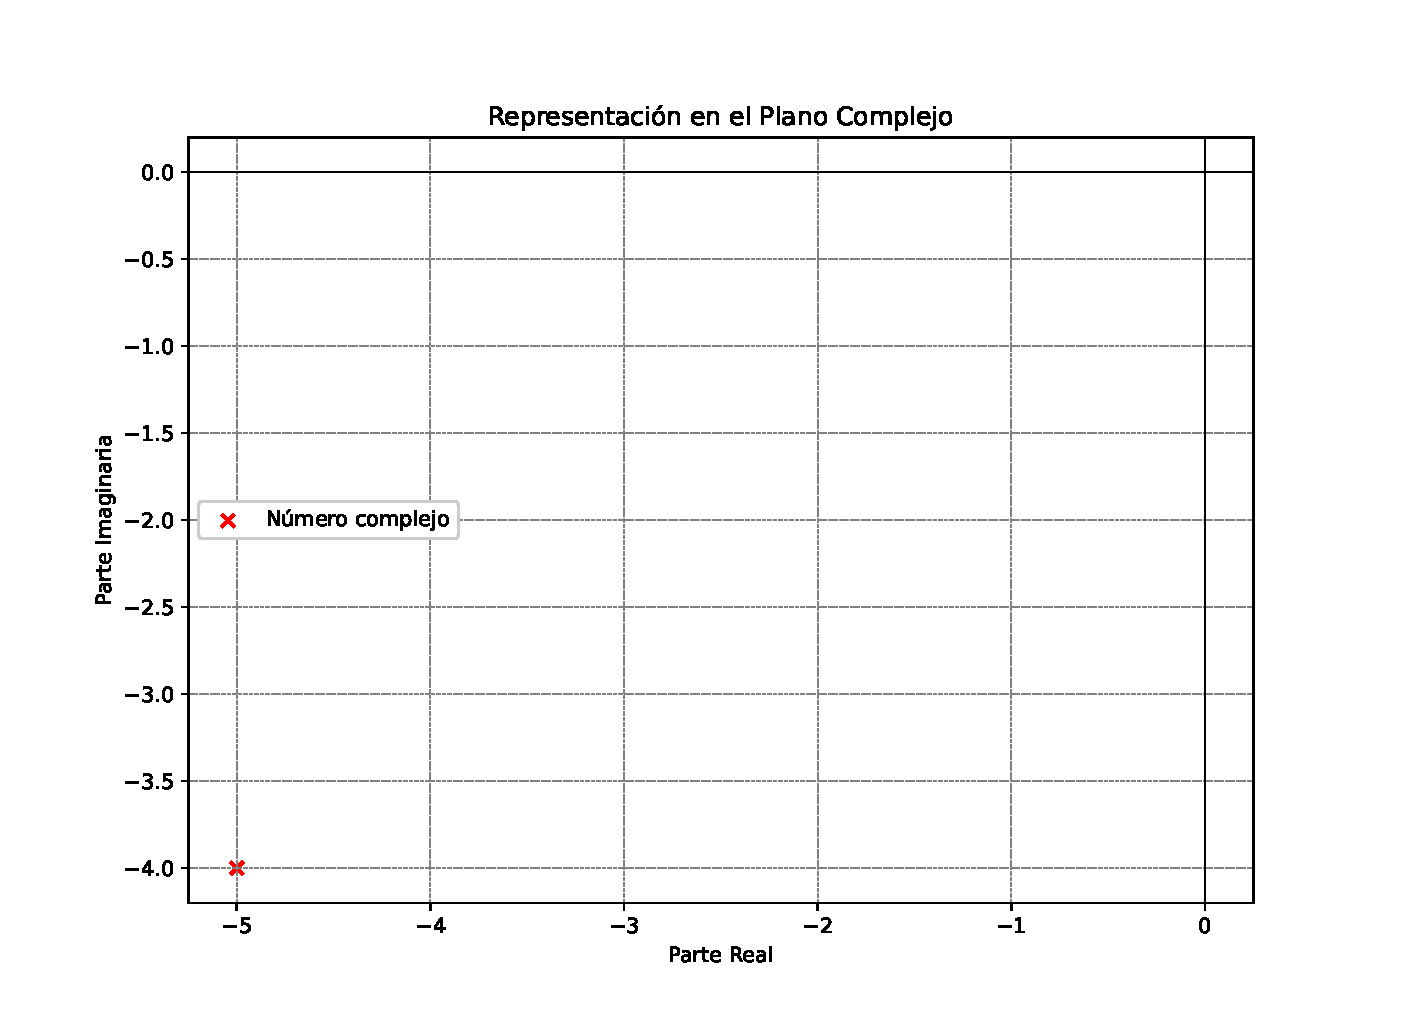
\includegraphics[scale=0.35]{representacioncomplejo.eps}
\caption{Representación gráfica en \texttt{matplotlib} del complejo $-5-4i.$}
\end{figure}

Estos resultados confirman los cálculos realizados en los problemas \ref{formageometrica54i} y \ref{formapolar54i}.
\end{myproof}
\end{prob}

\begin{prob} Sea $z$ un número complejo. Es posible probarse que si $\abs{z}=1,$ con $z\neq 1$ entonces $z=\dfrac{1+it}{1-it},$ con $t\in \mathbb{R}.$  Para el complejo $z=\dfrac{1}{2}+\dfrac{\sqrt{3}}{2}i$ se tiene que  $it$ es igual a %real
				\begin{multicols}{4}
					\begin{enumerate}[$(a)$]
						\item $ \dfrac{ 1-\sqrt{3}}{-3-\sqrt{3}}.$  
						\item $ \dfrac{-1+\sqrt{3}i}{1-\sqrt{3}i}.$  
						\item $ \dfrac{-1+\sqrt{3}}{3+\sqrt{3}}.$  %ok
						\item Ninguna.
					\end{enumerate}
				\end{multicols}							
\begin{myproof}
Observe que si $z=\dfrac{1+it}{1-it},$ entonces 
\begin{align*}
z\left( 1-it \right)&=1+it\\
z-zit&=1+it\\
z-1&=zit+it\\
\dfrac{z-1}{z+1}&=it.
\end{align*}

De esta manera, \begin{align*} it&=\dfrac{\dfrac{1}{2}+\dfrac{\sqrt{3}}{2}i-1}{\dfrac{1}{2}+\dfrac{\sqrt{3}}{2}i+1}=\dfrac{\dfrac{1}{2}+\dfrac{\sqrt{3}}{2}i-1}{\dfrac{1}{2}+\dfrac{\sqrt{3}}{2}i+1}\\
&=\dfrac{1+\sqrt{3}i-2}{1+\sqrt{3}i+2}=\boxed{\dfrac{-1+\sqrt{3}i}{3+\sqrt{3}i}}.
\end{align*}
Por lo cual, la opción correcta es \textbf{Ninguna.}
\end{myproof}
\end{prob}

\begin{prob}  (\cite{andreescu2014complex}, p. 30, Problema 5)
Sean $z_1 = 1+i$ y $z_2 = -1-i$. Encuentre el número complejo $z_3$ tal que el triángulo $z_1$, $z_2$ y $z_3$ sea equilátero.
\end{prob}

\begin{myproof}
El problema tiene dos soluciones, dependiendo del argumento a tomar. Se muestran ambas.

\begin{figure}[H]
\centering
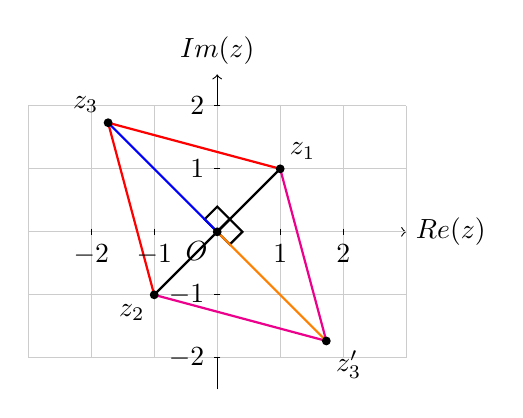
\begin{tikzpicture}[scale=0.8]
% Ejes
\draw[->] (-3,0) -- (3,0) node[right] {$\text{Re}(z)$};
\draw[->] (0,-2.5) -- (0,2.5) node[above] {$\text{Im}(z)$};

% Grilla
\draw[thin,gray!40] (-3,-2) grid (3,2);

% Marcadores de ángulo recto en el origen
\draw[thick] (0.2,0.2) -- (0,0.4) -- (-0.2,0.2) -- (0,0) -- cycle; 
\draw[thick] (0.2,-0.2) -- (0.4,0) -- (0.2,0.2) -- (0,0) -- cycle; 

% Lado principal z1-z2
\draw[thick] (-1,-1) -- (1,1);

% Primer triángulo equilátero
\draw[thick, red] (1,1) -- (-1.732,1.732);
\draw[thick, red] (-1.732,1.732) -- (-1,-1);

% Segundo triángulo equilátero
\draw[thick, magenta] (1,1) -- (1.732,-1.732);
\draw[thick, magenta] (1.732,-1.732) -- (-1,-1);

% Líneas desde el origen (alturas)
\draw[thick, blue] (-1.732,1.732) -- (0,0);
\draw[thick, orange] (1.732,-1.732) -- (0,0);

% Puntos
\fill[black] (1,1) circle (2pt);
\fill[black] (-1,-1) circle (2pt);
\fill[black] (-1.732,1.732) circle (2pt);
\fill[black] (0,0) circle (2pt);
\fill[black] (1.732,-1.732) circle (2pt);

% Etiquetas
\node[above right] at (1,1) {$z_1$};
\node[below left] at (-1,-1) {$z_2$};
\node[above left] at (-1.732,1.732) {$z_3$};
\node[below right] at (1.732,-1.732) {$z_3'$};
\node[below left] at (0,0) {$O$};

% Marcas en los ejes
\foreach \x in {-2,-1,1,2}
    \draw (\x,0.05) -- (\x,-0.05) node[below] {$\x$};
\foreach \y in {-2,-1,1,2}
    \draw (0.05,\y) -- (-0.05,\y) node[left] {$\y$};
\end{tikzpicture}
\caption{Representación gráfica de la solución}
\end{figure}



Observe que si $z_1 = 1+i$ y $z_2 = -1-i$ son vértices, entonces el segmento $\overline{z_1z_2}$ es un lado del triángulo. Como este es equilátero, su altura pasa por el punto medio del segmento, que es precisamente $0+0i$. 

La estrategia es calcular el módulo y argumento del complejo $z_3$ usando propiedades geométricas del triángulo equilátero.



\textbf{Cálculo del argumento:}

El argumento de $z_1$ es $\arg(z_1) = \arctan(1) = \frac{\pi}{4}$. 

Como la altura del triángulo equilátero es perpendicular al lado $\overline{z_1z_2}$, los posibles argumentos de $z_3$ son:
\begin{align}
\arg(z_3) &= \frac{\pi}{4} + \frac{\pi}{2} = \frac{3\pi}{4}\\
\arg(z_3') &= \frac{\pi}{4} - \frac{\pi}{2} = -\frac{\pi}{4} = \frac{7\pi}{4}
\end{align}

\textbf{Cálculo del módulo:}

La longitud del lado del triángulo es:
$$|z_1 - z_2| = |2 + 2i| = 2\sqrt{2}$$

En un triángulo equilátero, si el lado mide $a$, entonces la altura mide $\frac{\sqrt{3}}{2}a$. Por tanto:
$$|z_3| = \frac{\sqrt{3}}{2} \cdot 2\sqrt{2} = \sqrt{6}$$

\textbf{Soluciones finales:}

$$\boxed{z_3 = \sqrt{6} \cdot e^{i\frac{3\pi}{4}} = -\sqrt{3} + i\sqrt{3}}$$

$$\boxed{z_3' = \sqrt{6} \cdot e^{i\frac{7\pi}{4}} = \sqrt{3} - i\sqrt{3}}$$

\end{myproof}

De la multiplicación de números complejos en forma polar se derivan las siguientes propiedades importantes:

\begin{theorem}[Potencias y raíces enésimas de un número complejo] Sea $z=\abs{z}\mathrm{e}^{i\theta}$ un número complejo y $n$ un entero positivo, entonces:
\begin{enumerate}[$1.$]
\item $z^{n}=\abs{z}^n\mathrm{e}^{in\theta}$.
\item \textbf{Fórmula de De Moivre:} $\sqrt[n]{z}=\sqrt[n]{\abs{z}}\cdot \mathrm{e}^{i\frac{\theta+2k\pi}{n}}$ donde $k=0,1,\dots , n-1$.
\end{enumerate}
\end{theorem}

\begin{prob} Determine el valor de verdad de las siguientes afirmaciones donde $z$ y $w\ \in \mathbb{C}$. Si son verdaderas, demuéstrelas; de lo contrario, presente un contraejemplo.

\begin{multicols}{2}
\begin{enumerate}[$a)$]
       \item $z\overline{z}=|z|^2$.
      \item  $|z^n|=|z|^n$.
      \item  Si $\text{Re}(w)\neq 0$, $\text{arg}\left(\dfrac{z}{w}\right)=\dfrac{\text{arg}(z)}{\text{arg}(w)}$.
      \item  Si $z\in\mathbb{R}$, entonces $\text{arg}(z)=\pi$.
\end{enumerate}
\end{multicols}

\begin{myproof}	
\begin{enumerate}[$a)$]
\item Verdadero. \textbf{Demostración:}
Sea $z=a+bi$, entonces $\overline{z}=a-bi$. Por lo tanto:
$$z\overline{z}= (a+bi)(a-bi)= a^2 + abi - abi - b^2i^2 = a^2 + b^2 = |z|^2.$$

\item Verdadero. \textbf{Demostración:} 
Primero demostraremos que para cualesquiera números complejos $w$ y $z$, se cumple que $|wz|=|w||z|$.

Sean $w=a+ib$ y $z=c+di$. Entonces:
\begin{align*}
wz &= (a+ib)(c+di) = (ac-bd) + i(ad+bc)\\
|wz|^2 &= (ac-bd)^2 + (ad+bc)^2\\
&= a^2c^2 - 2abcd + b^2d^2 + a^2d^2 + 2abcd + b^2c^2\\
&= a^2(c^2+d^2) + b^2(c^2+d^2)\\
&= (a^2+b^2)(c^2+d^2)\\
&= |w|^2|z|^2
\end{align*}

Por lo tanto, $|wz| = |w||z|$.

Para demostrar que $|z^n|=|z|^n$ para todo entero positivo $n$, usamos inducción matemática:
- Base ($n=1$): Trivialmente, $|z^1|=|z|^1=|z|$.
- Paso inductivo: Supongamos que $|z^k|=|z|^k$ para algún $k \geq 1$.
- Para $n=k+1$: $|z^{k+1}| = |z^k \cdot z| = |z^k| \cdot |z| = |z|^k \cdot |z| = |z|^{k+1}$

Por el principio de inducción matemática, $|z^n|=|z|^n$ para todo entero positivo $n$.

\item Falso. \textbf{Contraejemplo:} 
Sea $z=1$ y $w=1+i$. 

Calculamos $\dfrac{z}{w} = \dfrac{1}{1+i} = \dfrac{1(1-i)}{(1+i)(1-i)} = \dfrac{1-i}{2}$.

Por lo tanto:
$$\text{arg}\left(\dfrac{z}{w}\right) = \text{arg}\left(\dfrac{1-i}{2}\right) = \text{arg}(1-i) = -\frac{\pi}{4} = \frac{7\pi}{4}$$

Mientras que:
$$\dfrac{\text{arg}(z)}{\text{arg}(w)} = \dfrac{\text{arg}(1)}{\text{arg}(1+i)} = \dfrac{0}{\frac{\pi}{4}} = 0$$

Como $\frac{7\pi}{4} \neq 0$, la afirmación es falsa.

\item Falso. \textbf{Contraejemplo:} 
Sea $z=1 \in \mathbb{R}$. Entonces $\text{arg}(z) = 0 \neq \pi$. 

En realidad, para cualquier número real positivo $z > 0$, tenemos $\text{arg}(z) = 0$, y para cualquier número real negativo $z < 0$, tenemos $\text{arg}(z) = \pi$. La afirmación solo es cierta para números reales negativos.
\end{enumerate}
\end{myproof}
\end{prob}

\begin{prob}  (\cite{andreescu2014complex}, p. 55, Problemas 1 y 3) Use la fórmula de De Moivre para encontrar las raíces cuartas de los siguientes complejos:
\begin{multicols}{2}
\begin{enumerate}[$a)$]
\item $z=-27$.
\item $z=-7+24i$.
\end{enumerate}
\end{multicols}
\begin{myproof}
Para calcular las raíces cuartas de los números complejos dados, primero los expresaremos en forma polar y luego aplicaremos la fórmula de De Moivre.

\begin{enumerate}[$a)$]
\item Para $z=-27$:
   
   El módulo es $|-27| = 27$ y su argumento es $\text{arg}(-27) = \pi$, por lo cual, $z = 27\cdot e^{i\pi}$.
   
   Las raíces cuartas están dadas por:
   $$\sqrt[4]{z} = \sqrt[4]{27}\cdot \mathrm{e}^{i\frac{\pi+2k\pi}{4}}$$
   donde $k=0,1,2,3$.
   
   Dado que $\sqrt[4]{27} \approx 2.28$, tenemos:
   $$\begin{matrix}
   k=0: & \sqrt[4]{27}\cdot\mathrm{e}^{i\frac{\pi}{4}} &\approx& 2.28\cdot\mathrm{e}^{i\frac{\pi}{4}} &\approx& 1.61+1.61i \\
   k=1: & \sqrt[4]{27}\cdot\mathrm{e}^{i\frac{3\pi}{4}} &\approx& 2.28\cdot\mathrm{e}^{i\frac{3\pi}{4}} &\approx& -1.61+1.61i \\
   k=2: & \sqrt[4]{27}\cdot\mathrm{e}^{i\frac{5\pi}{4}} &\approx& 2.28\cdot\mathrm{e}^{i\frac{5\pi}{4}} &\approx& -1.61-1.61i \\
   k=3: & \sqrt[4]{27}\cdot\mathrm{e}^{i\frac{7\pi}{4}} &\approx& 2.28\cdot\mathrm{e}^{i\frac{7\pi}{4}} &\approx& 1.61-1.61i
   \end{matrix}$$

\item Para $z=-7+24i$:
   
   El módulo es $|z| = \sqrt{(-7)^2+(24)^2} = \sqrt{49+576} = \sqrt{625} = 25$.
   
   Para el argumento, como $z$ está en el segundo cuadrante (parte real negativa, parte imaginaria positiva):
   $$\text{arg}(z) = \arctan\left(\frac{24}{-7}\right) + \pi = \arctan(-\frac{24}{7}) + \pi \approx -1.2863 + \pi \approx 1.8553 \text{ radianes}$$
   
   Por lo tanto, $z = 25\cdot e^{i\cdot 1.8553}$.
   
   Las raíces cuartas están dadas por:
   $$\sqrt[4]{z} = \sqrt[4]{25}\cdot \mathrm{e}^{i\frac{1.8553+2k\pi}{4}}$$
   donde $k=0,1,2,3$ y $\sqrt[4]{25} = 2.24$
   
   $$\begin{matrix}
   k=0: & 2.24\cdot\mathrm{e}^{i\frac{1.8553}{4}} &\approx& 2.24\cdot\mathrm{e}^{i\cdot 0.4638} &\approx& 2.02+0.94i \\
   k=1: & 2.24\cdot\mathrm{e}^{i\frac{1.8553+2\pi}{4}} &\approx& 2.24\cdot\mathrm{e}^{i\cdot 2.0344} &\approx& -0.68+2.14i \\
   k=2: & 2.24\cdot\mathrm{e}^{i\frac{1.8553+4\pi}{4}} &\approx& 2.24\cdot\mathrm{e}^{i\cdot 3.6050} &\approx& -2.02-0.94i \\
   k=3: & 2.24\cdot\mathrm{e}^{i\frac{1.8553+6\pi}{4}} &\approx& 2.24\cdot\mathrm{e}^{i\cdot 5.1756} &\approx& 0.68-2.14i
   \end{matrix}$$
\end{enumerate}
\end{myproof}
\end{prob}

\section{Teorema Fundamental del Álgebra}

\begin{definition}[Raíz de un polinomio] 
Sea $p(z)$ un polinomio con coeficientes complejos. Diremos que $\alpha \in \mathbb{C}$ es una raíz de $p(z)$ si $p(\alpha)=0$. Es decir, $\alpha$ es una solución de la ecuación polinómica $p(z)=0$.
\end{definition}

El cálculo de las raíces de un polinomio puede ser un problema muy difícil y se estudia ampliamente en matemáticas, en una rama llamada análisis numérico. Debido a los alcances de este curso, se tratarán polinomios especiales con coeficientes complejos (que incluyen los de coeficientes reales como caso particular) para los cuales sea fácil calcular su factorización. Sin embargo, el siguiente teorema no distingue el tipo de polinomio a estudiar. Este teorema es un resultado muy importante demostrado, entre otros, por \textbf{Carl Friedrich Gauss} (1777--1855), un célebre matemático alemán que nombraremos bastante en este curso.

\begin{theorem}[Teorema Fundamental del Álgebra]\label{tfam}
Todo polinomio no constante $p(z)$ de grado $n \geq 1$ con coeficientes complejos tiene exactamente $n$ raíces en $\mathbb{C}$, contando sus multiplicidades algebraicas.
\end{theorem}

\begin{rem}
La multiplicidad algebraica de una raíz $\alpha$ de un polinomio $p(z)$ es el mayor entero positivo $m$ tal que $(z-\alpha)^m$ divide a $p(z)$. En otras palabras, es el exponente más alto de $(z-\alpha)$ en la factorización completa de $p(z)$. Por ejemplo, si $p(z) = (z-1)^2(z-2)$, entonces $z=1$ es una raíz con multiplicidad algebraica $2$, mientras que $z=2$ es una raíz con multiplicidad algebraica $1$ (o raíz simple). En adelante, cuando se haga referencia a la multiplicidad de una raíz, se entenderá la multiplicidad algebraica ya que luego en la Definición \ref{multiplicidadgeometrica} exténderemos este concepto.
\end{rem}

\begin{prob}(\cite{andreescu2014complex}, p. 55, Problema 7) Use la fórmula de De Moivre para encontrar todas las raíces complejas de los siguientes polinomios:

\begin{multicols}{2}
\begin{enumerate}[$a)$]
\item $z^4-z^2+1=0$
\item $z^7-2iz^4-iz^3-2=0$
\end{enumerate}
\end{multicols}

\begin{myproof}
\begin{enumerate}[$a)$]
\item Tome $w=z^2$ entonces la ecuación se reduce a $w^2-w+1=0$. Usando la fórmula cuadrática las soluciones son  $$w = \frac{-(-1)\pm\sqrt{(-1)^2-4(1)(1)}}{2(1)} = \frac{1\pm\sqrt{-3}}{2} = \frac{1\pm i\sqrt{3}}{2}$$

Note que las soluciones son números complejos, además que $w$ es raíz cuadrada de $z$, por lo cual se calcula la forma polar de cada complejo y sus raíces cuadradas:

\begin{itemize}
\item Para $w=\frac{1+\sqrt{3}i}{2}$:  

$|w| = \sqrt{\left( \frac{1}{2} \right)^2 + \left( \frac{\sqrt{3}}{2} \right)^2} = \sqrt{\frac{1}{4}+\frac{3}{4}} = 1,$ y $\arg(w) = \arctan\left( \frac{\sqrt{3}/2}{1/2} \right) = \arctan(\sqrt{3}) = \frac{\pi}{3}.$


Las raíces cuadradas son $\sqrt{1} e^{i\frac{\frac{\pi}{3}+2k\pi}{2}}$ donde $k=0,1$.

$k=0:   e^{i\frac{\pi/3}{2}} = \boxed{e^{i\frac{\pi}{6}}}$ y $k=1: e^{i\frac{\pi/3+2\pi}{2}} = \boxed{e^{i\frac{7\pi}{6}}}$

\item Para $w=\frac{1-i\sqrt{3}}{2}$:

$|w| = \sqrt{\left( \frac{1}{2} \right)^2 + \left( \frac{\sqrt{3}}{2} \right)^2} = 1$ y $\arg(w) = \arctan\left( \frac{-\sqrt{3}/2}{1/2} \right) = \arctan(-\sqrt{3}) = -\frac{\pi}{3}$


Tomando el argumento principal: $\arg(w) = 2\pi - \frac{\pi}{3} = \frac{5\pi}{3}$.

Las raíces cuadradas son $\sqrt{1} e^{i\frac{\frac{5\pi}{3}+2k\pi}{2}}$ donde $k=0,1$.

$k=0:  e^{i\frac{5\pi/3}{2}} = \boxed{e^{i\frac{5\pi}{6}}}$ y  $k=1: e^{i\frac{5\pi/3+2\pi}{2}} = \boxed{e^{i\frac{11\pi}{6}}}$
\end{itemize}

Finalmente las soluciones de la ecuación son:
$$z_1 = e^{i\frac{\pi}{6}}, \quad z_2 = e^{i\frac{5\pi}{6}}, \quad z_3 = e^{i\frac{7\pi}{6}}, \quad z_4 = e^{i\frac{11\pi}{6}}$$

\item Factorizando la ecuación: $z^7-2iz^4-iz^3-2=z^4(z^3-2i)-i(z^3-2i)=(z^4-i)(z^3-2i)= 0.$

Como los complejos forman un dominio entero, la ecuación se puede resolver calculando los valores de $z$ tales que $z^4=i$ y $z^3=2i$.

\begin{itemize}
\item Para $z^4=i$: $|i|=1$ y $\arg(i)=\frac{\pi}{2}$.

Las raíces cuartas son $e^{i\frac{\frac{\pi}{2}+2k\pi}{4}}$ donde $k=0,1,2,3$.

$k=0:\boxed{e^{i\frac{\pi}{8}}},$ $k=1: \boxed{e^{i\frac{5\pi}{8}}},$ $k=2: \boxed{e^{i\frac{9\pi}{8}}},$ $k=3: \boxed{e^{i\frac{13\pi}{8}}}.$

\item Para $z^3=2i$: $|2i|=2$ y $\arg(2i)=\frac{\pi}{2}$.

Las raíces cúbicas son $\sqrt[3]{2} e^{i\frac{\frac{\pi}{2}+2k\pi}{3}}$ donde $k=0,1,2$.

$k=0: \boxed{\sqrt[3]{2}e^{i\frac{\pi}{6}}},$ $k=1: \boxed{\sqrt[3]{2}e^{i\frac{5\pi}{6}}},$ $k=2: \boxed{\sqrt[3]{2}e^{i\frac{3\pi}{2}}}.$
\end{itemize}

Finalmente las soluciones de la ecuación son:
$z_1 = e^{i\frac{\pi}{8}},$ $z_2 = e^{i\frac{5\pi}{8}},$ $z_3 = e^{i\frac{9\pi}{8}},$ $z_4 = e^{i\frac{13\pi}{8}},$ $z_5 = \sqrt[3]{2}e^{i\frac{\pi}{6}},$ $z_6 = \sqrt[3]{2}e^{i\frac{5\pi}{6}},$ $z_7 = \sqrt[3]{2}e^{i\frac{3\pi}{2}}.$
\end{enumerate}
\end{myproof}
\end{prob}



\section{Problemas propuestos para el capítulo}

\begin{prob} Determine cuál opción es correcta y justifique por qué las demás son incorrectas:

El efecto geométrico de multiplicar por el complejo $w=6\left(\dfrac{3+3i}{3-3i}\right)$ en el plano complejo es:
%\begin{multicols}{2}
\begin{enumerate}[$(a)$]
\item sextuplicar el módulo y girar $\dfrac{\pi}{2}$ en sentido horario.
\item duplicar el módulo y girar $\pi$ en sentido antihorario.
\item multiplicar el módulo por $3$ y girar $\dfrac{\pi}{4}$ en sentido horario.
\item multiplicar el módulo por $6$ y girar $\pi$ en sentido antihorario.
\item Ninguna.					
\end{enumerate}
%\end{multicols}
\end{prob}



\begin{prob}\label{compsombreado}
Determine cuál opción es correcta y justifique por qué las demás son incorrectas.

El subconjunto de números complejos sombreado en la gráfica es:


\begin{figure}[H]
\centering 		
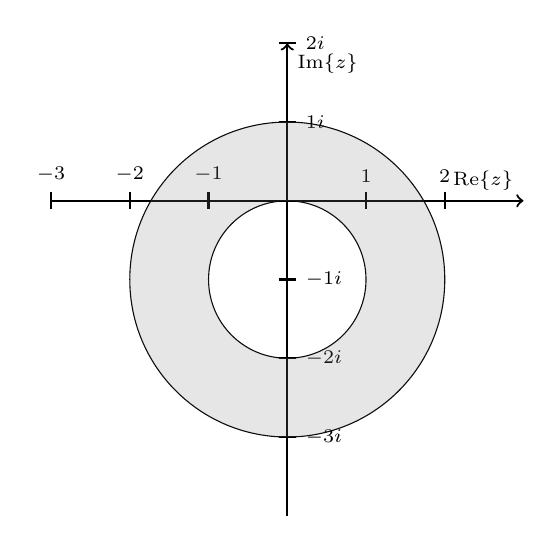
\begin{tikzpicture}
\begin{scope}[thick,font=\scriptsize][set layers]
\draw [->] (-3,0) -- (3,0) node [above left]  {Re$\{z\}$};
    \draw [->] (0,-4) -- (0,2) node [below right] {Im$\{z\}$};
    \foreach \n in {-3,...,-1,1,2}{%
        \draw (\n,-3pt) -- (\n,3pt)   node [above] {$\n$};
        \draw (-3pt,\n) -- (3pt,\n)   node [right] {$\n i$};
    }
    \end{scope}
    \draw[solid] (0,-1) circle (1);
    \draw[solid] (0,-1) circle (2);
    \path [draw=none, fill=gray, even odd rule, fill opacity = 0.2] (0,-1) circle (2) (0,-1) circle (1);
\end{tikzpicture}
\caption{Figura del problema \ref{compsombreado}}
\end{figure} 
\begin{multicols}{2}
\begin{enumerate}[$(a)$]
\item  $\left\lbrace z\in \mathbb{C}: 1\leq\abs{z-i}\leq 2 \right\rbrace$
\item  $\left\lbrace z\in \mathbb{C}:  \abs{z-(-i)}\leq 2 \right\rbrace$
\item $\left\lbrace z\in\mathbb{C}:1\leq|z-(-i)|\leq 2\right\rbrace$
\item  $\left\lbrace z\in \mathbb{C}:  \abs{z-i}\leq 2 \right\rbrace$
\end{enumerate}
\end{multicols}
\end{prob}

\begin{prob} En el plano complejo, represente el conjunto de números complejos $z$ tales que:
$$\dfrac{4\pi}{6}\leq\text{arg}(z)\leq\dfrac{5\pi}{6} \text{ y } |z|<3$$
\end{prob}

\begin{prob}[Examen 1 - Preliminares, semestre 2019 - 2] \label{compubicacion}
En el plano complejo se han dibujado los números complejos $z$ y $w$ como se muestra en la figura. Indique en la misma figura dónde quedarían aproximadamente los números: 

\begin{multicols}{2}
\begin{enumerate}[$a)$]
\item $\dfrac{1}{z}$
\item $(1+i)z$
\item $\overline{w}$ 
\item $-z$ 
\item $w^2$
\end{enumerate}		
		
\begin{figure}[H]
\centering
\begin{tikzpicture}[scale=1.5]
    % Ejes coordenados
    \draw[->] (-1.3,0) -- (1.5,0) node[above left] {Re};
    \draw[->] (0,-1.35) -- (0,1.75) node[below right] {Im};
    
    % Marcas en los ejes
    \draw (1,-2pt) -- (1,2pt) node[above] {$1$};
    \draw (-2pt,1) -- (2pt,1) node[right] {$i$};
    
    % Círculo unitario punteado
    \draw[dashed] (0,0) circle (1);
    
    % Vector z (primer cuadrante, 45°)
    \draw[->, thick] (0,0) -- (0.707,0.707);
    \node at (0.7,0.8) {$z$};
    
    % Vector w (segundo cuadrante)
    \draw[->, thick] (0,0) -- (-0.355,0.352);
    \node at (-0.5,0.5) {$w$};
    
\end{tikzpicture}
\caption{Figura del problema \ref{compubicacion}}
\end{figure}
\end{multicols}
\end{prob}
	
\begin{prob}[Examen 1 - Preliminares, semestre 2019 - 2] 
La ecuación $2z^4+2z^2+1=0$ tiene una raíz compleja $z$ con argumento entre $\pi$ y $\dfrac{3\pi}{2}$. Determine el argumento de $z$.
\end{prob}		

\begin{prob}[Examen 1 - Preliminares, semestre 2022 - 2] 
Use la fórmula de De Moivre para encontrar todas las raíces complejas del polinomio $z^6-11(i+1)z^3+121i=0$.
\end{prob}

\begin{prob} 
Determine el valor de verdad de las siguientes afirmaciones donde $z, w \in \mathbb{C}$. Si son verdaderas demuéstrelas; si son falsas, muestre un contraejemplo.

\begin{enumerate}[$a)$]
\item  $|z|=|iz|$
\item  Si $z$ y $w$ son imaginarios puros, entonces $zw$ es imaginario puro.
\item  Si $z\neq \mathbf{0}$, entonces $\left|\dfrac{z}{|z|}\right|=1$
\item  Si $re^{i\theta}$ es la forma polar de $z$, entonces $\text{Im}(z)=r\sin \theta$
\item $\arg(z)=-\arg(\overline{z})$
\item  Si $z$ y $\overline{z}$ son raíces de $ax^2+bx+c=0$, entonces $b^2-4ac<0$
\item  Sean $z, w\in \mathbb{C}$. Si $|w|<1$ y $|z|\leq 1$, entonces $\left|\dfrac{z+w}{1+\overline{w}z}\right|=1$
\item  Si $z$ y $w$ son imaginarios puros, entonces $zw\in \mathbb{R}$
\item  $z=\overline{z}$ si y solo si $z$ es real
\item  Si $z$ es imaginario puro, entonces $z^{-1}=-z$
\item  Si $\overline{z}=-z$, entonces $z$ es imaginario puro
\item  Si $z=a+bi$ con $a=b$, entonces $|z|=|a|\sqrt{2}$
\item  Si $z=bi$ con $b\neq 0$, entonces $iz$ es real
\end{enumerate}
\end{prob}

\begin{prob} 
(\cite{andreescu2014complex}, p. 19, Problema 9) Encuentre los números reales $x, y$ en cada caso:

\begin{enumerate}[$a)$]
\item $(1-2i)x + (1+2i)y=1+i$
\item $(4-3i)x^2+(3+2i)xy=4y^2-\dfrac{1}{2}x^2+(3xy-2y^2)i$
\end{enumerate}
\end{prob}

\begin{prob} 
(\cite{andreescu2014complex}, p. 21, Problema 31) Sean $z_1, z_2, z_3$ números complejos tales que $z_1+z_2+z_3=0$ y $|z_1|=|z_2|=|z_3|=1$. Demuestre que $z_1^2+z_2^2+z_3^2=0$.
\end{prob}

\begin{prob} 
Encuentre la forma polar de los siguientes números complejos. ¿Cuál es el efecto geométrico de multiplicar y dividir por cada uno? Justifique su respuesta.

\begin{multicols}{3}
\begin{enumerate}[$a)$]
\item $z=3+i$
\item $z=5-i$
\item $z=8$
\end{enumerate}
\end{multicols}
\end{prob}

\begin{prob}  
(\cite{andreescu2014complex}, p. 55, Problema 5) Use la fórmula de De Moivre para encontrar las raíces cuartas de:
\begin{multicols}{2}
\begin{enumerate}[$a)$]
\item $z=-27$
\item $z=-7+24i$
\end{enumerate}
\end{multicols}
\end{prob}

\begin{prob}  
(\cite{andreescu2014complex}, p. 55, Problema 7) Use la fórmula de De Moivre para encontrar todas las raíces complejas de:
\begin{multicols}{2}
\begin{enumerate}[$a)$]
\item $z^4+16=0$
\item $z^3-27i=0$
\item $z^5-1-i=0$
\item $(2-3i)z^6+1+5i=0$
\item $z^{10}+(-2+i)z^5-2i=0$
\end{enumerate}
\end{multicols}
\end{prob}

\begin{prob} 
Demuestre que $z$ es imaginario puro si y solo si $z=-\overline{z}$.
\end{prob}